\documentclass[12pt]{article}
\usepackage{hyperref}
\usepackage{natbib}
\usepackage{amsmath}
\usepackage{nicefrac}
\usepackage[usenames,dvipsnames]{xcolor}
\usepackage{graphicx}
\usepackage{footnote}
\usepackage{rotating}
%\usepackage{slashbox}
\usepackage{afterpage}
\usepackage{float}
\usepackage{color}

\usepackage[margin = 1.0 in]{geometry}
\usepackage{natbib}

\renewcommand{\bottomfraction}{.9}
\renewcommand{\topfraction}{.9}
\renewcommand{\textfraction}{0.1}
\renewcommand{\floatpagefraction}{.9}


%%%%%%%%%%%%%%%%%%%%%%%%%%%%%%%%%%%%%%%%%%%%%%%%%%%%%%%%%%%%%%%%%%%%%%%%%%%%
%   document style macros
%%%%%%%%%%%%%%%%%%%%%%%%%%%%%%%%%%%%%%%%%%%%%%%%%%%%%%%%%%%%%%%%%%%%%%%%%%%%
\def\gtrsim{\mathrel{\hbox{\rlap{\hbox{\lower4pt\hbox{$\sim$}}}\hbox{$>$}}}}
\def\lessim{\mathrel{\hbox{\rlap{\hbox{\lower4pt\hbox{$\sim$}}}\hbox{$<$}}}}
\newcommand{\ddg}{$\Delta\Delta G~$}
%%%%%%%%%%%%%%%%%%%%%%%%%%%%%%%%%%%%%%%%%%%%%%%%%%%%%%%%%%%%%%%%%%%%%%%%%%%%

\graphicspath{{../figures/}}

\title{Sequence variability as the main determinant of sequence-structure relationships}
\author{Amir Shahmoradi$^{1*}$, Eleisha L. Jackson$^2$, Claus O. Wilke$^2$}
\begin{document}

\date{\today}
\maketitle


\noindent
$^1$ Department of Physics, The University of Texas at Austin, Austin, TX 78712, USA \\
$^2$ Institute of Cellular and Molecular Biology, Center for Computational Biology and Bioinformatics, and Department of Integrative Biology, The University of Texas at Austin, Austin, Texas, 78712 USA\\

\bigskip
\noindent
$^*$Corresponding author\\
$\phantom{^*}$Email: amir@physics.utexas.edu\\
%$\phantom{^*}$Phone:{ \color{red} Need a phone} \\
$\phantom{^*}$Phone: +1 512 232 2459\\

\bigskip
\noindent
Manuscript type: research article\\
\bigskip
\noindent  Keywords: protein evolution, relative solvent accessibility, site variability


\begin{abstract}
NEED TO EDIT THE ABSTRACT\\
Recent work has shown that structural properties are capable of predicting site-specific sequence variability for a given protein. However, the strength and significance of these structure-sequence relations appear to vary widely among different proteins, with absolute correlation strengths ranging from $0.1$ to $0.8$.  Here we present the results from a comprehensive search for potential biophysical and structural determinants of protein evolution by studying more than $200$ structural and evolutionary properties in a dataset of $209$ monomeric enzymes. We discuss the main protein characteristics responsible for the general patterns of protein evolution, and identify sequence divergence as the main determinant of the strengths of virtually all structural-evolution relationships, explaining $10-30 \%$ of observed variation in sequence-structure relations. In addition to sequence divergence, we identify several protein structural properties that are moderately but significantly coupled with the strength of sequence-structure relations. In particular, proteins with more homogeneous back-bone hydrogen bond energies, large fractions of helical secondary structures and low fraction of beta sheets tend to have the strongest correlations between structural properties and site variability. 

\end{abstract}
\vfill
\vfill
\def\thefootnote{\fnsymbol{footnote}}
\setcounter{footnote}{0}


\section{Introduction}
\label{sec:intro}

Proteins are subject to a number of biophysical and functional constraints \citep{Scherreretal2012, Wilkeetal2010}. These constraints result site-specific patterns of sequence variability within a protein. Recently several site-specific structural properties that can explain patterns of sequence variability in proteins have been identified. One of the earliest examples is Relative Site Accessibility. \cite{Fransozaetal2009} identified RSA as the strongest predictor of evolutionary rate. They found that residues that are buried in the core of proteins tend to be more conserved than exposed residues close to the surface of the protein. In their analysis these concerned both RSA and various definitions of residue packing density to predict evolutionary rate. They found that RSA and evolutionary rate shared a significant linear relationship. Afterwards, several other works \citep{Ramseyetal2011, Scherreretal2012} also found that RSA as a very significant predictor of evolutionary rate and found this linear relationship as well. However in these papers all have the same flaw. During the course of their analysis they binned the protein sites and average over all sites within a bin when looking at the trend of RSA. This could produce artifacts when looking at the trend. \\
\indent Later, Yeh et al performed a similar analysis on a series of enzyme monomer proteins and found that packing density, as defined by CN and WCN \citep{Liaoetal2005, Yehetal2014, Huangetal2014}, was the strongest determinant of site variability. A year later, Sharamoradi et al also performed a site-wise analysis on a series of viral proteins. In this analysis they found that RSA had the strongest correlation with site variability. Additionally the effect seen between CN and WCN was of a much smaller magnitude as compared to \citep{Yehetal2014}. Here we attempt to reconcile the work done in this area. We find that site variability is the primary determinant of structure determinant of the strength of structure-sequence relationships and some differences in previous work can be explained in terms of differing levels of site variability. \\
COPY EDIT THIS!!! \\


\section{Materials and Methods}
\label{sec:mam}

    \subsection*{Structures, sequences, and measures of sequence properties } 
    The results presented in this work are based on a two datasets. The first is a dataset of $209$ monomeric enzymes from \citep{Echaveetal2015} originally from Huang et al. (2014).The original dataset was comprised of $213$ but we removed four of the proteins (1BBS, 1BS0, 1DIN, 2HPL) that had did not have data at insertion sites. Briefly, these proteins are all enzyme monomers   randomly picked from the Catalytic Site Atlas $2.2.11$ \citep{Porteretal2004} with protein sizes in the sample ranging from $95$ to $1287$. For each structure we had a corresponding alignment of up to 300 homologous sequences.  The second dataset was from taken from Sharamoradi et al. and is comprised of nine? viral proteins. The viral proteins range from 122 - 557 in length and each structure is accompanied by a sequence alignment of up to 2362 homologous sequences. Sequence alignments for both datasets constructed using amino-acid sequences with MAFFT \citep{Katohetal2002, Katohetal2005}, specifying the auto flag to select the optimal algorithm for the given data set.The alignments were then used to calculate the site-specific evolutionary rates for each individual protein in both datasets. To do so, we relied on two independent methods of measuring sequence variability measure. First, we calculated the Shannon entropy ($H_i$) -- the sequence entropy, hereafter abbreviated as {\it seqent} -- at each alignment column $i$:
    \begin{equation}
        \label{eqn:shannon}
        H_i = -\sum_j P_{ij}\ln P_{ij}
    \end{equation}

    where $P_{ij}$ is the relative frequency of amino acid $j$ at position $i$ in the alignment. The sequence entropy is a measure of variability at each site. We also calculated a measure of site-specific evolutionary rate -- hereafter abbreviated as {\it r4s} -- for each protein using software Rate4site. First the Maximum Likelihood phylogenetic trees were inferred with RAxML, using the LG substitution matrix and the CAT model of rate heterogeneity \citep{Stamatakis2006, Stamatakis2014}. For each structure, we then used the respective sequence alignment and phylogenetic tree to infer site-specific substitution rates with Rate4Site, using the empirical Bayesian method and the amino-acid Jukes-Cantor mutational model (aaJC) \citep{Mayroseetal2004}.

    \subsection*{Calculation of Structural Properties}
    
    HOW IS CN and WCN Defined and Calculated??? (Cite Shih et al for WCN) Possbily Lin Paper \\
\indent We used DSSP \citep{Kabschetal2005}  for the calculation of Accessible Surface Area (ASA) for each site. We normalized the ASA for each site by the theoretical maximum solvent accessibility values of \cite{Tienetal2013}  to obtain the Relative Solvent Accessibility (RSA) for all individual sites in all proteins. In addition to ASA values, we also extract from DSSP output, information about the secondary structure of proteins such as the total number of residues participating in different types of helices, parallel or anti-parallel beta sheets, or loops and turns. To complete the list of pdb-level structural properties, we also calculate the Spearman correlations between all residue-level structure and sequence properties and include them in the analysis to probe their potential effects on the strength of structure-sequence relations. \\

All data and analysis scripts required to reproduce the work are publicly available to view and download at \url{https://github.com/shahmoradi/cordiv}.


\section{Results}
\label{sec:results}

    \subsection*{}
{\color{red}SOME RESULTS.....} \\


\section{Discussion}
\label{sec:dcr}
{\color{red}SOME DISCUSSION.....} \\


\section{Acknowledgements}
The authors acknowledge the Texas Advanced Computing Center (TACC) at The University of Texas at Austin for providing High-performance computing resources. ELJ is is funded by a National Science Graduate Research Fellowship, grant number DGE-1110007. COW is funded by {\color{red} Which grants??}.  AS is funded by {\color{red} Which grants??}.
....

%\clearpage
%\newpage

%\cleardoublepage

\bibliographystyle{peerj} %"style
\bibliography{manuscript_bib} %expected file "my refs.bib"

\cleardoublepage
\section*{Figures}

    \begin{figure}[H]
            \centerline{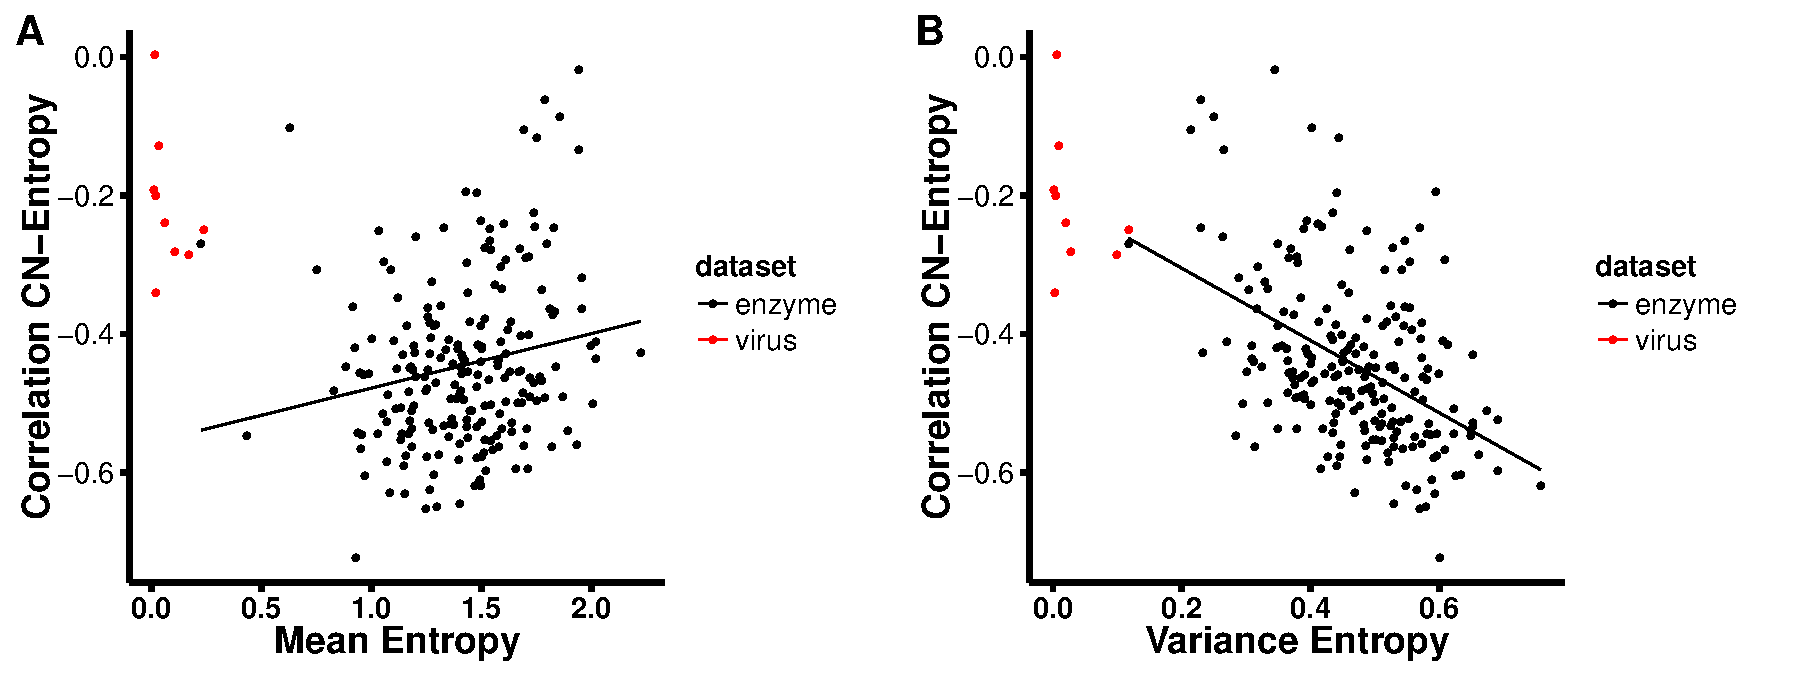
\includegraphics[width=7.5in]{entropy_cn_cor.pdf}}     
            \caption{NEED A CAPTION!!!.}
            \label{fig:seqent_structure_cors}
    \end{figure}


    \begin{figure}[H]
            \centerline{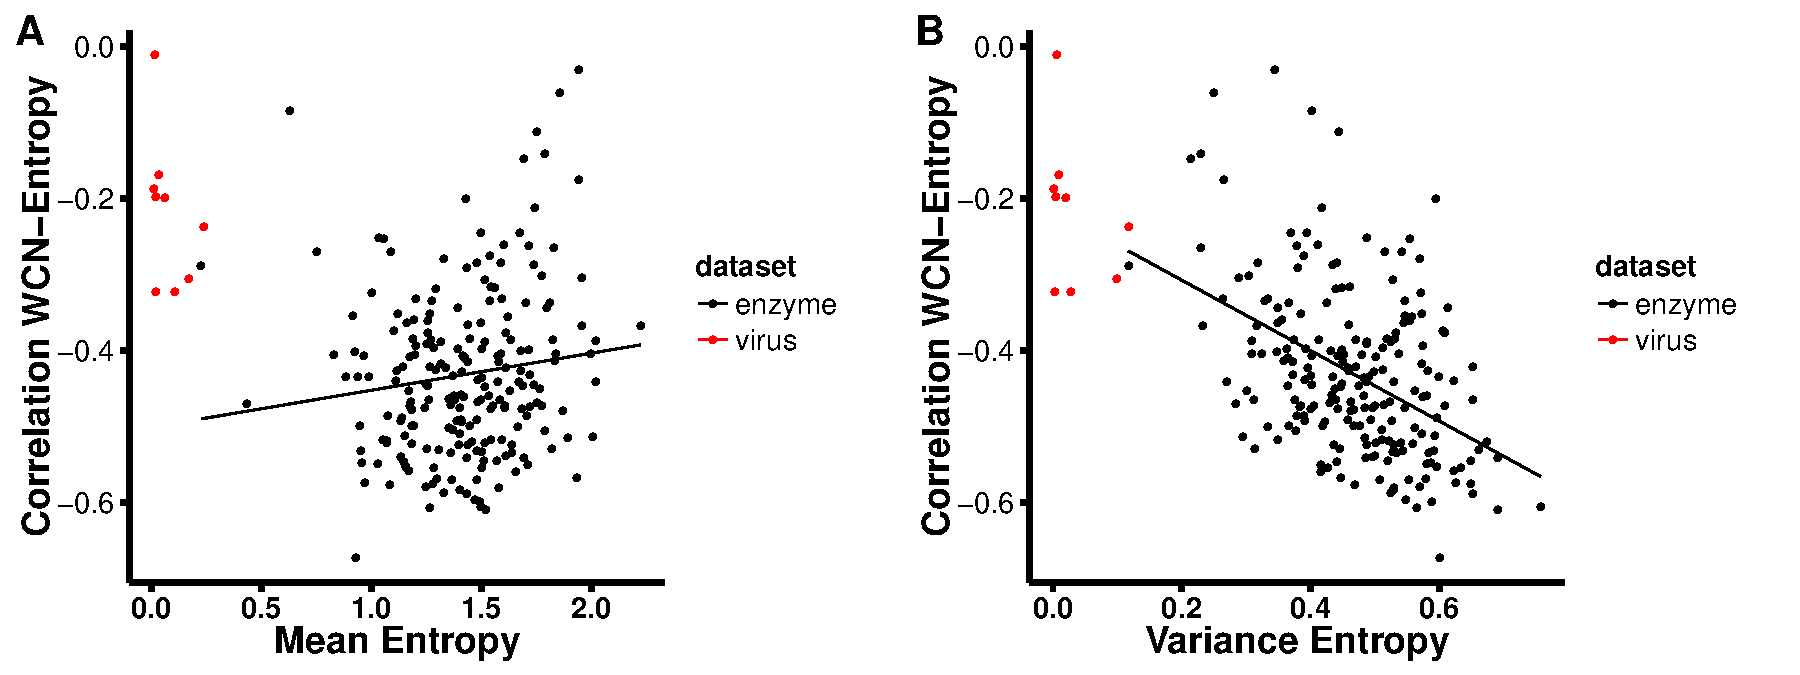
\includegraphics[width=7.5in]{entropy_wcn_cor.pdf}}     
            \caption{NEED A CAPTION!!!.}
            \label{fig:seqent_structure_cors}
    \end{figure}


    \begin{figure}[H]
            \centerline{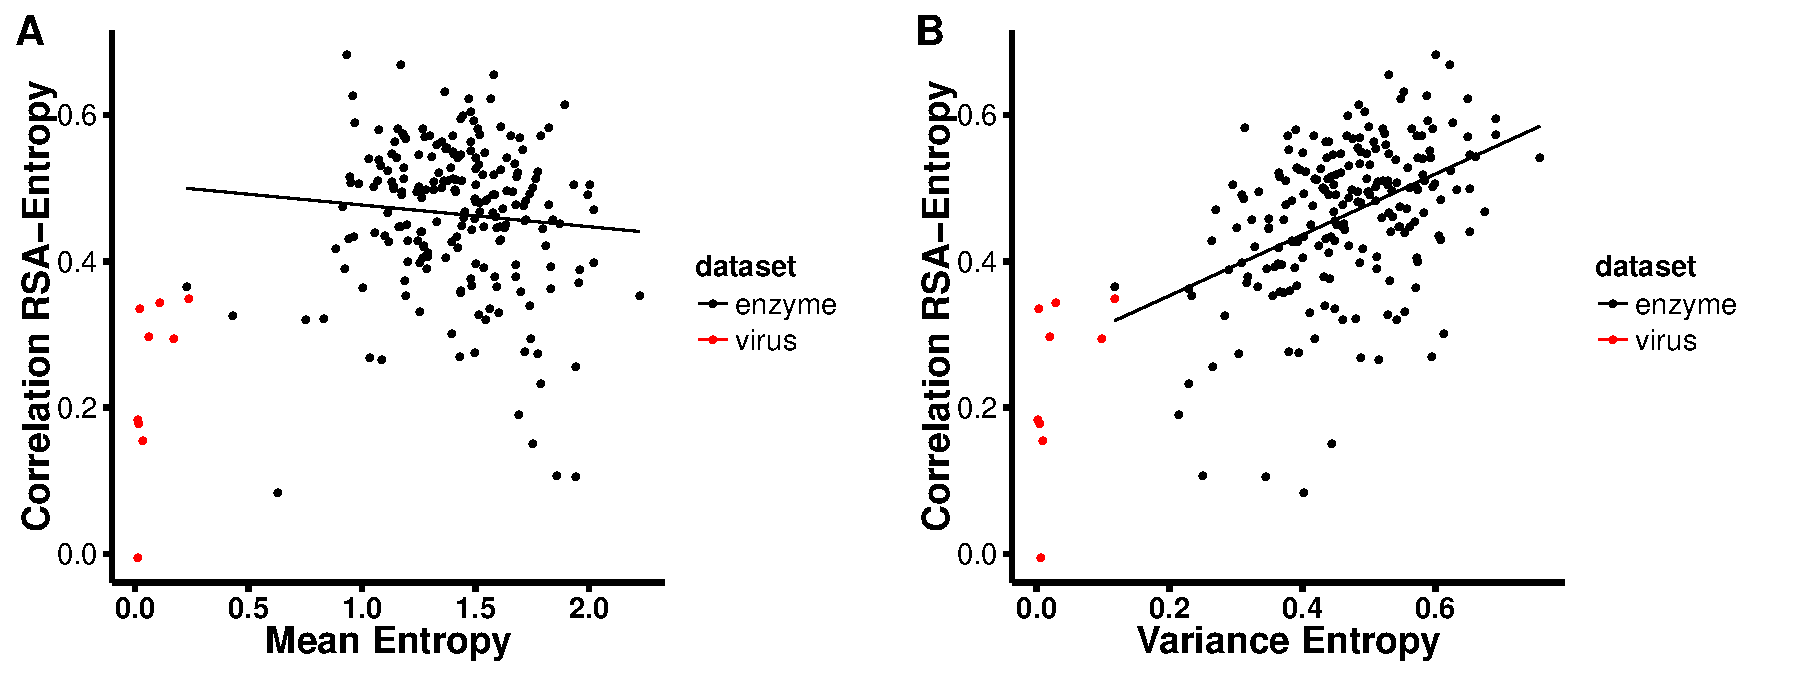
\includegraphics[width=7.5in]{entropy_rsa_cor.pdf}}     
            \caption{NEED A CAPTION!!!.}
            \label{fig:seqent_structure_cors}
    \end{figure}
  
       
        \begin{figure}[H]
            \centerline{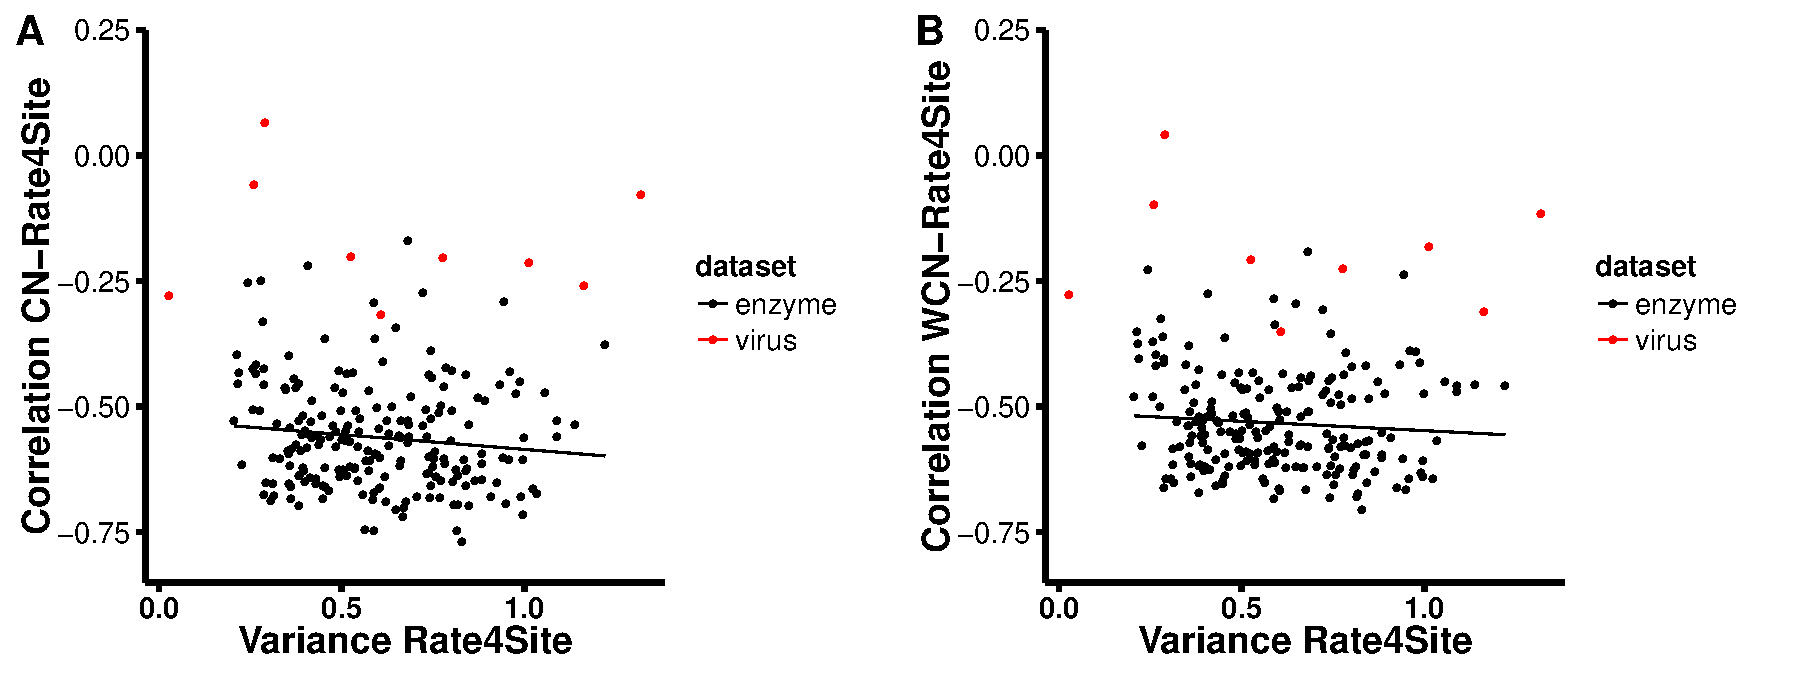
\includegraphics[width=7.5in]{rate_cor.pdf}}     
            \caption{NEED A CAPTION!!!.}
            \label{fig:seqent_structure_cors}
    \end{figure}
    
    
            \begin{figure}[H]
            \centerline{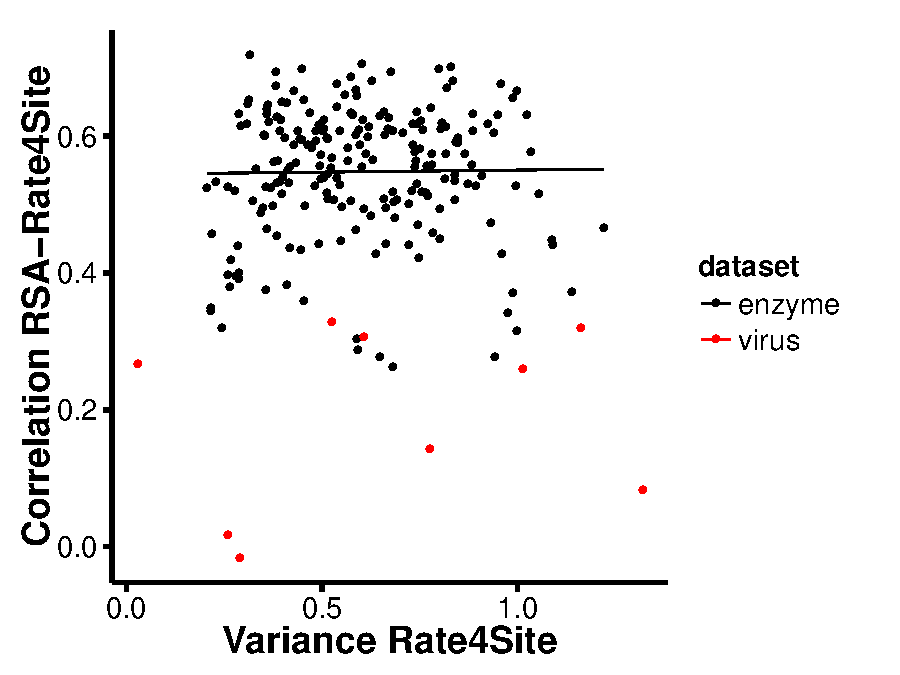
\includegraphics[width=5.0in]{var_rate_rsa_cor.pdf}}     
            \caption{NEED A CAPTION!!!.}
            \label{fig:seqent_structure_cors}
    \end{figure}
    
        \begin{figure}[H]
            \centerline{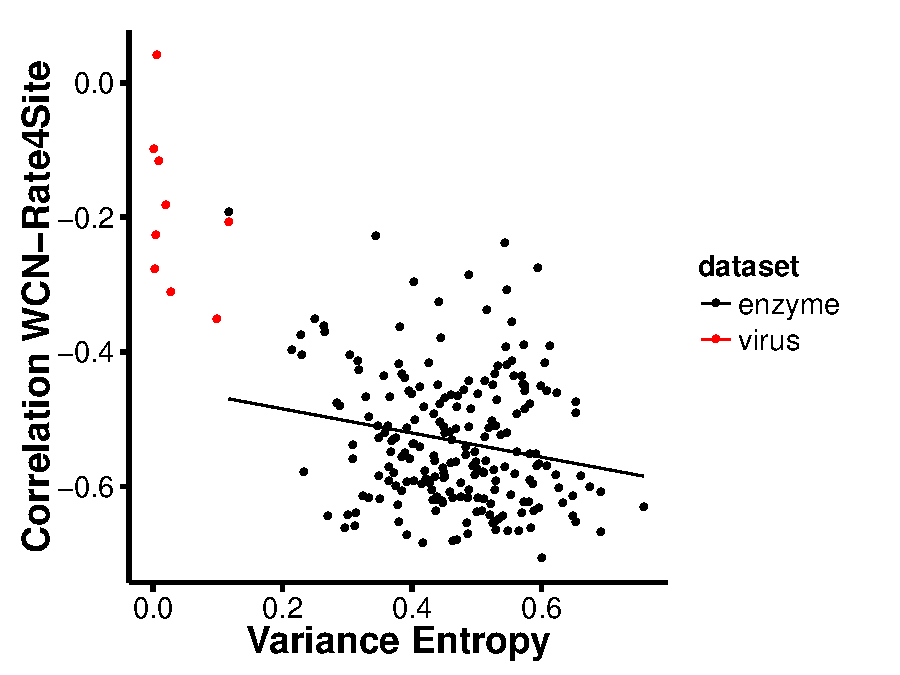
\includegraphics[width=5.0in]{var_entropy_rate_cor.pdf}}     
            \caption{NEED A CAPTION!!!.}
            \label{fig:seqent_structure_cors}
    \end{figure}
    


\end{document}

